\documentclass[cjk,dvipdfmx,12pt,%
hyperref={bookmarks=true,bookmarksnumbered=true,bookmarksopen=false,%
colorlinks=false,%
pdftitle={野良ビルドから始めるパッケージ作成},%
pdfauthor={佐々木洋平},%
%pdfinstitute={uwabami@debian.or.jp},%
pdfsubject={第37回関西Debian勉強会 at OSC 2010 Kansai$@$kyoto},%
}]{beamer}

\title{野良ビルドから始めるパッケージ作成}
\subtitle{{\scriptsize{$\sim$第37回関西Debian勉強会 at OSC 2010 Kansai$@$kyoto$\sim$}}}
\author[佐々木 洋平]{{\large\bf 佐々木洋平}}
\institute[Debian JP]{{\normalsize\tt uwabami@debian.or.jp}}
\date{{\small 2010 年 7 月 10 日}}

%\usepackage{amsmath}
%\usepackage{amssymb}
\usepackage{graphicx}
\usepackage[varg]{txfonts}
%\usepackage{D6math}
\AtBeginDvi{\special{pdf:tounicode EUC-UCS2}}
\usetheme{Kyoto}
\def\museincludegraphics{%
  \begingroup
  \catcode`\|=0
  \catcode`\\=12
  \catcode`\#=12
  \includegraphics[width=0.9\textwidth]}
%\renewcommand{\familydefault}{\sfdefault}
%\renewcommand{\kanjifamilydefault}{\sfdefault}
\begin{document}
\settitleslide
\begin{frame}
\titlepage
\end{frame}
\setdefaultslide




\takahashi[50]{こんにちは}


\begin{frame}[fragile]
\frametitle{はじめる前に}

\begin{itemize}
\item 当セッションでは,
後半で Live DVD/USB を用いた
パッケージ作成実習を行ないます.

\begin{itemize}
\item Live DVD/USB を受け取ってない方は申し出て下さい.
\item 数量限定/品切れ御免
\end{itemize}
\item 受け取った方は試しに boot してみて下さい.

\begin{itemize}
\item 起動しなかったらゴメンナサイ
\end{itemize}
\end{itemize}

\end{frame}

\begin{frame}[fragile]
\frametitle{おことわり/disclaimer}


\begin{itemize}
\item 毎度毎度の無保証です

\begin{itemize}
\item 用法, 用量を守って正しくお使い下さい
\end{itemize}
\item 疑問/質問/茶々/ツッコミ大歓迎

\begin{itemize}
\item 遠慮なくどうぞ.
\end{itemize}
\end{itemize}


\end{frame}


\begin{frame}[fragile]
\frametitle{発表者について}


\begin{columns}[t]
\column{0.6\paperwidth}

\begin{description}
\item[名前] \mbox{}

\textbf{佐々木洋平}
\item[IRC] \mbox{}

uwabami
\item[所属] \mbox{}

Debian JP Project\\地球流体電脳倶楽部
\item[連絡先] \mbox{}

\verb|uwabami@debian.or.jp|\\u\verb|wabami@gfd-dennou.org|
\end{description}

\column{0.4\paperwidth}

\begin{figure}[h]
\centering\museincludegraphics{./image201007/mattari.png}|endgroup
\end{figure}

\end{columns}


\end{frame}


\takahashi[50]{話のまくら}


\begin{frame}[fragile]
\frametitle{Debian Package's Life Cycle}



\begin{figure}[h]
    \centering
    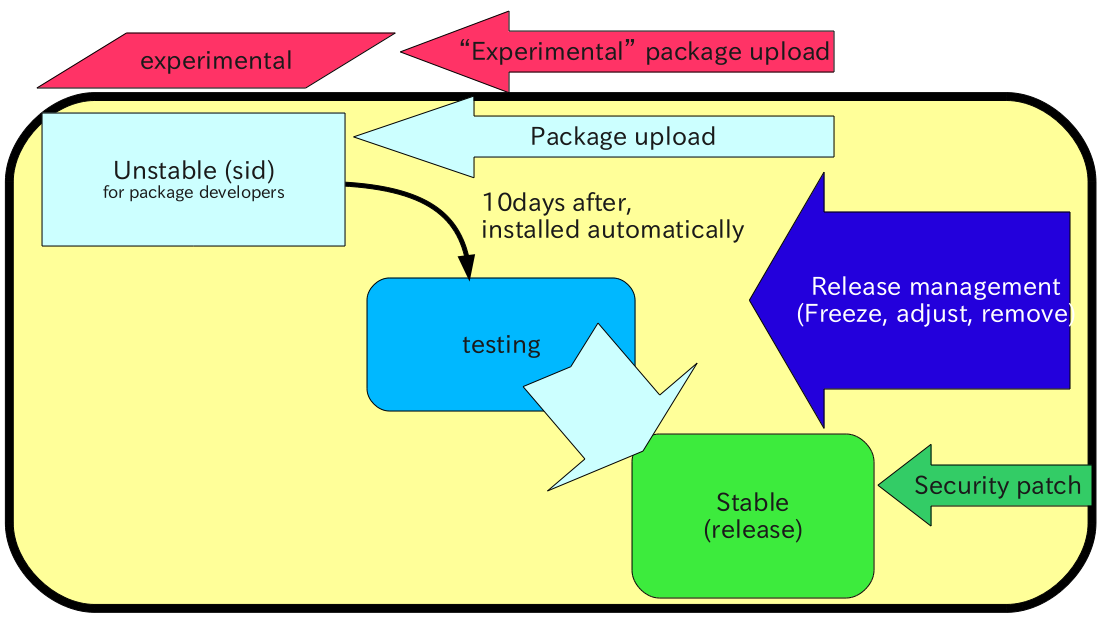
\includegraphics[width=1.05\textwidth]{%
      ./image201007/201007-debian-development-cycle.png}
\end{figure}


\end{frame}
\begin{frame}[fragile]
\frametitle{Freeze is comming\dots{}}


\begin{itemize}
\item 当初は 3 月?
\item ミラー障害とかあって, 5 月末 or 6 月に変更

\begin{itemize}
\item 移行/修正が終わらないアレやコレがあって\dots{}
\end{itemize}

\item 多分 8 月に \textbf{freeze}

\item 年内リリース?

\begin{itemize}
\item またバレンタインになったりして.
\end{itemize}
\end{itemize}


\end{frame}


\takahashi[20]{...そうは言っても...}
\takahashi[20]{魅力的なソフトウェア}


\begin{frame}[fragile]
\frametitle{例(1) ibuz-mozc}


\begin{columns}[t]
\column{0.55\paperwidth}

\begin{description}
\item[ibus-mozc] \mbox{}

open-source project originates from \textbf{Google Japanese Input}.
\end{description}

\begin{itemize}
\item ITP: Bug\#581158

\begin{itemize}
\item もうすぐ unstable に入るYo!
\end{itemize}
\end{itemize}

\column{0.4\paperwidth}

\begin{figure}[h]
\centering\museincludegraphics{./image201007/201007-mozc-icon.png}|endgroup
\end{figure}

\end{columns}


\end{frame}

\begin{frame}[fragile]
\frametitle{例(2) chromium-browser}


\begin{columns}[t]
\column{0.55\paperwidth}

\begin{description}
\item[chromium-browser] \mbox{}

Chromium is an open-source browser project originates from \textbf{Chrome}.
\end{description}

\column{0.4\paperwidth}

\begin{figure}[h]
\centering\museincludegraphics{./image201007/201007-chromium-icon.png}|endgroup
\end{figure}

\end{columns}

\begin{itemize}
\item unstable なら apt 一発
\end{itemize}

\begin{quote}
\begin{verbatim}
% apt-get install chromium-browser
\end{verbatim}
\end{quote}

\end{frame}

\takahashi[20]{魅力的な更新}

\begin{frame}[fragile]
\frametitle{魅力的な更新}


\begin{itemize}
\item emacs \textbf{23}
\item gnome \textbf{2.30}
\item KDE \textbf{4}
\item ruby \textbf{1.9.1}
\item python 2.6
\end{itemize}

\dots{}

\end{frame}

\takahashi[50]{最新の○○が使いたい!}


\begin{frame}[fragile]
\frametitle{\dots{}}


\begin{columns}[t]
\column{0.45\paperwidth}
\begin{figure}[h!]
    \centering
    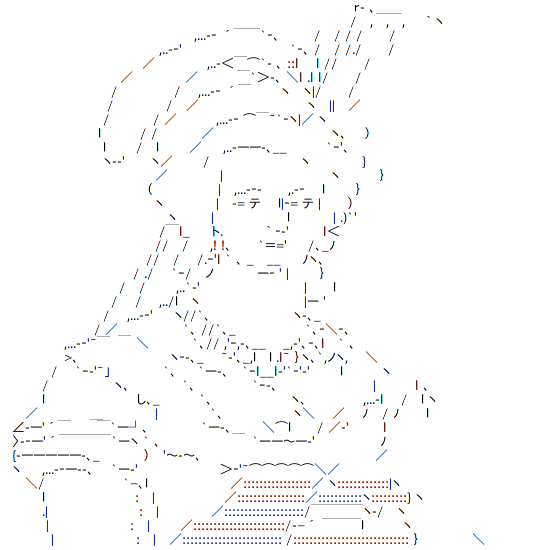
\includegraphics[width=1.05\textheight]{./image201007/AA-MarieAntoinette.png}
\end{figure}


\column{0.45\paperwidth}

\begin{center}
stable に無いなら unstable を使えば良いじゃない.
\end{center}

\end{columns}


\end{frame}


\takahashi[50]{でも unstable は{\normalsize{ちょっと}}怖い!?}
\takahashi[50]{そんな貴方に}


\begin{frame}[fragile]
\frametitle{Agenda}


\begin{itemize}
\item 座学

\begin{enumerate}
\item Debian Backports の紹介
\item apt の「ピン止め」
\end{enumerate}

\item 実習: Backports hands on
\end{itemize}


\end{frame}

\section{Debian Backports の紹介}


\takahashi[50]{{\tt Debian Backports}}


\begin{frame}[fragile]
\frametitle{Debian Backports}


\begin{center}
\underline{\url{http://www.backports.org}}
\end{center}

\begin{itemize}
\item testing, unstableのソースを\\
stable 向けに再コンパイルしたパッケージを提供

\begin{itemize}
\item security-update にも対応

\item 公式な安定版よりも新しいバージョンが使える, かも
\end{itemize}

\item 普段は stable を使っているけれども,
特定のソフトウェアは新しいバージョンを使用したい時にオススメ
\end{itemize}


\end{frame}

\begin{frame}[fragile]
\frametitle{backports を使うなら\dots{}(1)}

\begin{itemize}
\item apt-line に以下を追加
\end{itemize}

\begin{commandline}
deb http://www.backports.org/debian lenny-backports main contrib non-free
\end{commandline}

\begin{itemize}
\item 更新 \& target を指定して install
\end{itemize}

\begin{commandline}
% sudo apt-get update
% sudo apt-get install emacs23 -t lenny-backports
\end{commandline}


\end{frame}

\begin{frame}[fragile]
\frametitle{backports を使うなら\dots{}(2)}


\begin{itemize}
\item apt-get upgrade すると

\begin{itemize}
\item lenny-backports のパッケージに upgrade される
\end{itemize}
\item それが嫌なら \textbf{apt のピン止め} を行なうべし
\end{itemize}


\end{frame}


\takahashi[50]{apt の\\「ピン止め」}



\begin{frame}[fragile]
\frametitle{apt のピン止め}


\begin{itemize}
\item 特定のパッケージ/リリースに対して \textbf{優先度} を設定
\item 優先度に応じて, apt がパッケージを処理する.

\begin{itemize}
\item インストール対象にしない
\item 明示的に指定すればインストール可能\\
アップグレードの対象にはならない
\item ダウングレードしてでも, そのリリースを install する
\begin{center}
\dots{}などなど
\end{center}
\end{itemize}
\end{itemize}


\end{frame}


\begin{frame}[fragile]
\frametitle{apt pin の優先度}

\begin{tabular}{ll}
優先度 & 意味 \\
\hline
0 & install しない \\
1--99 & 指定すれば install 可能 \\
 & upgrade の対象にはならない \\
100 & 現在 install されているパッケージ \\
(500) & 現在 install されていないパッケージ \\
(989) & apt-pin の default \\
990 & apt-get の target-release が指定されている場合 \\
1000 以上 & ダウングレードしてもそのパッケージを install \\
\end{tabular}
\end{frame}

\begin{frame}[fragile]
\frametitle{backports 用の pin止めの例}


/etc/apt/preferences に以下の用に書くと?


\begin{commandline}
Package: *
Pin: release a=lenny-backports
Pin-Priority: 99
\end{commandline}

\begin{itemize}
\item release が lenny-backports の
\item 全てのパッケージ (*) を
\item 優先度 99 にピン止め

\begin{itemize}
\item 明示的に指定すればインストール可能
\item アップグレードの対象にはしない
\end{itemize}
\end{itemize}


\end{frame}


\begin{frame}[fragile]
\frametitle{さらに pin 止めしてみると}

\begin{itemize}
\item apt-line に testing/unstable があっても安心
\end{itemize}

\begin{commandline}
Package: *
Pin: release a=lenny-backports
Pin-Priority: 99

Package: *
Pin: release a=testing
Pin-Priority: 98

Package: *
Pin: release a=unstable
Pin-Priority: 97
\end{commandline}


\end{frame}


\takahashi[30]{欲しいパッケージが \\backports に無いよ?}



\begin{frame}[fragile]
\frametitle{\dots{}}


\begin{columns}[t]
\column{0.45\paperwidth}
\begin{figure}[h!]
    \centering
    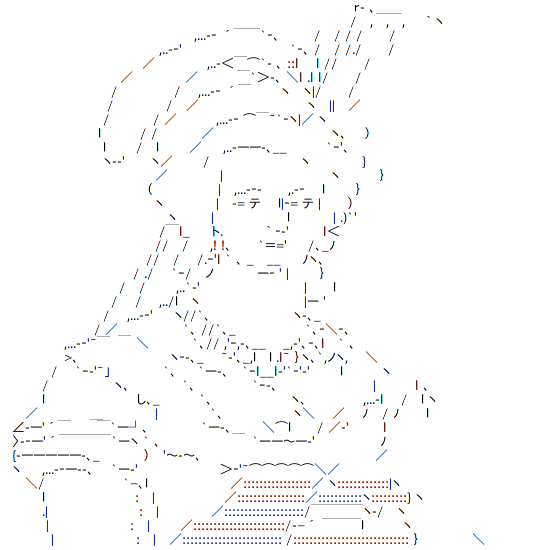
\includegraphics[width=1.05\textheight]{./image201007/AA-MarieAntoinette.png}
\end{figure}


\column{0.45\paperwidth}

\begin{center}
backports に無いなら\dots{}ry)
\end{center}

\end{columns}


\end{frame}


\takahashi[50]{ではなくて}
\takahashi[40]{野良 backports を作ろう!}


\begin{frame}[fragile]
\frametitle{野良 backports の作り方}


\begin{itemize}
\item 材料

\begin{enumerate}
\item 安定版の動いているマシン
\item testing/unstable の \textbf{ソースパッケージ}
\end{enumerate}

\item レシピ

\begin{enumerate}
\item apt の pin 止めをする
\item apt-get source \textbf{パッケージ名} -t testing(unstable)
\item 依存するパッケージを install してパッケージ作成

\begin{itemize}
\item パッケージが古くて依存関係が満たせない\\
→ 2. に戻ってくりかえし
\end{itemize}
\end{enumerate}
\end{itemize}


\end{frame}


\takahashi[50]{実習その1: zsh}



\begin{frame}[fragile]
\frametitle{実習その1: zsh}

\begin{itemize}
\item 何故?

\begin{itemize}
\item (個人的に) \textbf{vcs\textunderscore{}info} が使いたかったから
\end{itemize}
\end{itemize}

\begin{description}
\item[vcs\textunderscore{}info] \mbox{}

VCS の情報を PROMPT に出す zsh の関数

\begin{itemize}
\item lenny の zsh には無い
\item 良い大人は
「その関数だけ自前で持てば」なんて言わない
\end{itemize}
\end{description}


\end{frame}


\begin{frame}[fragile]
\frametitle{下準備}


\begin{itemize}
\item ネットワークがありません!
\item 以下のファイルの apt-line をコメントアウト!

\begin{itemize}
\item /etc/apt/sources.list
\item /etc/apt/sources.list.d/debian-backports\textunderscore{}lenny.list
\item /etc/apt/sources.list.d/sid-source.list
\end{itemize}
\item /etc/apt/sources.list.d/osckyoto.list を有効に

\begin{itemize}
\item /live 以下のローカルリポジトリを使用
\end{itemize}
\end{itemize}

\end{frame}

\begin{frame}[fragile]
\frametitle{ソースの取得}


\begin{commandline}
% sudo apt-get update
% apt-get source zsh -t unstable
\end{commandline}


\end{frame}

\begin{frame}[fragile]
\frametitle{依存するパッケージのインストール}


\begin{commandline}
% sudo apt-get build-dep zsh
パッケージリストを読み込んでいます... 完了
依存関係ツリーを作成しています
状態情報を読み取っています... 完了
以下のパッケージが新たにインストールされます:
  libcap-dev libcap1 libkpathsea4 libncursesw5-dev libpcre3-dev
  libpcrecpp0 tex-common texi2html texinfo texlive-base texlive-base-bin
  texlive-common texlive-doc-base texlive-latex-base
アップグレード: 0 個、新規インストール: 14 個、削除: 0 個、保留: 10 個。
13.6MB 中 0B のアーカイブを取得する必要があります。
この操作後に追加で 44.4MB のディスク容量が消費されます。
...
\end{commandline}


\end{frame}

\begin{frame}[fragile]
\frametitle{パッケージのビルド}

\begin{itemize}
\item 単に rebuild するだけならば
\end{itemize}

\begin{commandline}
% cd zsh-4.3.10
% dch --bpo
% debuild -rfakeroot -uc -us
...
\end{commandline}


\end{frame}


\takahashi[50]{実習その2: qwit}


\begin{frame}[fragile]
\frametitle{実習その2: qwit}


\begin{description}
\item[qwit] \mbox{}

Qt を使った twitter client
\end{description}

\begin{itemize}
\item 何故 qwit?

\begin{itemize}
\item のがたさんのオススメだから
\item lenny の qwit は古い
\item 良い大人は
「非公式 RT が\dots{}」とか「QT って\dots{}」\\なんて言わない

\begin{itemize}
\item でも佐々木は使っていないが.
\end{itemize}
\end{itemize}
\end{itemize}

\end{frame}


\takahashi[25]{やってみよう!}




\takahashi[50]{実習その3: Arora}


\begin{frame}[fragile]
\frametitle{実習その3: Arora}


\begin{description}
\item[Arora] \mbox{}

Qt4 + webkit な Web browser

\begin{itemize}
\item HTML5 ready!
\item 軽い!/速い!/美しい!
\end{itemize}
\end{description}

\end{frame}


\takahashi[50]{依存解決が\\大変です(笑)}
\takahashi[50]{宿題, \\ということで}


\begin{frame}[fragile]
\frametitle{宿題/お土産}


\begin{itemize}
\item 今回の Live DVD/USB

\begin{itemize}
\item lenny 用の Arora + 依存パッケージを同梱
\end{itemize}

\item uim のバグ有

\begin{itemize}
\item 日本語入力を試みると Arora は落ちます
\item uim or scim を backports?
\end{itemize}
\end{itemize}

\end{frame}


\begin{frame}[fragile]
\frametitle{参考文献}

\begin{itemize}
\item \url{http://backports.org/dokuwiki/doku.php}
\item \url{http://jaqque.sbih.org/kplug/apt-pinning.html}
\item マリーアントワネットの AA の作者\@2ch
\end{itemize}

\end{frame}


\takahashi[50]{ }































\end{document}
%%% Local Variables:
%%% mode: japanese-latex
%%% TeX-master: t
%%% End:
